\documentclass[a4paper,12pt]{article} % тип документа

% report, book

% Рисунки
\usepackage{graphicx}
\usepackage{wrapfig}
\usepackage{mathtext}
\usepackage[left=2cm,right=2cm,
    top=2cm,bottom=2cm,bindingoffset=0cm]{geometry}

\usepackage{hyperref}
\usepackage[rgb]{xcolor}
\hypersetup{				% Гиперссылки
    colorlinks=true,       	% false: ссылки в рамках
	urlcolor=blue          % на URL
}

%  Русский язык
\usepackage[T2A]{fontenc}			% кодировка
\usepackage[utf8]{inputenc}			% кодировка исходного текста
\usepackage[english,russian]{babel}	% локализация и переносы
\addto\captionsrussian{\def\refname{Список используемой литературы}}


% Математика
\usepackage{amsmath,amsfonts,amssymb,amsthm,mathtools} 
\usepackage{titlesec}
\titlelabel{\thetitle.\quad}

\usepackage{wasysym}

\begin{document}\begin{titlepage}

\thispagestyle{empty}

\centerline{МОСКОВСКИЙ ФИЗИКО-ТЕХНИЧЕСКИЙ ИНСТИТУТ}
\centerline{(НАЦИОНАЛЬНЫЙ ИССЛЕДОВАТЕЛЬСКИЙ УНИВЕРСИТЕТ)}

\vfill

\centerline{\huge{Лабораторная работа 3.3.4}}
\centerline{\LARGE{<<Эффект Холла в полупроводниках>>}}

\vfill

Студент группы Б02-109 \hfill Назарчук Анна

\vfill

\centerline{Долгопрудный, 2022}
\clearpage
\end{titlepage} 

\section{Аннотация}
В работе изучен эффект Холла для полупроводников, рассчитана подвижность носителей заряда. Измерения проведены с помощью мостика Холла на образце легированного германия. Получены зависимости холловского напряжения от индукции магнитного поля, вычислено значение подвижности частицы, сходящееся с табличным. 

\section{Введение}
Электрический ток окружает человека повсюду и представляет собой направленный перенос зарядов с помощью микрочастиц - носителей заряда. Проводимость большинства твердых тел связана с движением электронов. Несмотря на то, что электроны входят в состав всех тел, некоторые не проводят электрический ток, а другие являются хорошими проводниками. Более того, существуют материалы, которые ведут себя так, будто вместо электронов ток в них переносят положительные частицы (называемые дырками); бывают даже вещества (обозначаемые полупроводниками), которые имеют два типа носителей: электроны и дырки. Но как хорошо они проводят электрический ток, насколько подвижны носители заряда, как много их в таких материалах? На эти вопросы и хотелось ответить в данной работе.


\section{Методика измерений}
Наиболее современным и удобным методом изучения полупроводников являются способы на основе эффекта Холла:

Во внешнем магнитном поле $B$ на заряды $q$ действует сила Лоренца $F$:
\begin{equation}
F = qE+qu\times B,  \hspace{2mm}
\end{equation}
 $u$ - средняя скорость движения, $E$ - напряженность электрического поля
Эта сила вызывает движение носителей. Действительно, траектории частиц будут либо искривляться, либо, если геометрия проводника этого не позволяет,
возникнет дополнительное электрическое поле, компенсирующее магнитную
составляющую силы Лоренца. В этом и заключается суть эффекта Холла. 
Рассмотрим связь между электрическим полем $E$ и плотностью тока $j$ (параметры, которые можно получить экспериментально). Пусть $B$ направлено по оси $z$, сила Лоренца при движении носителей с постоянной средней скоростью будет уравновешена трением (\cite{labnik}):
\begin{equation}
q(E+u\times B)-\frac{qu}{\mu}=0
\end{equation}
$\mu$ - подвижность носителей тока.
Откуда:
\begin{equation}
\label{mu}
E = 
 \begin{pmatrix}
 1 & -\mu B & 0\\
 \mu B & 1 & 0\\
 0 & 0 & 1\\
 \end{pmatrix}
 \frac{j}{\sigma_0}, \hspace{2mm} \sigma_0 = qn\mu
\end{equation}
$n$ - концентрация носителей.
Для исследования полупроводников использована схема, называемая мостиком Холла (рис. \ref{мостик}), ее параметры: ширина пластинки $a$, толщина $h$,
длина $l$.
\begin{figure}[h!]
\begin{center}
\includegraphics[width=0.55\textwidth]{мостик}
\caption{Мостик Холла - схема для исследования влияния магнитного поля на проводящие свойства} \label{мостик}
\end{center}
\end{figure} 
Холловское напряжение равно:
\begin{equation}
\label{R_H}
U_\perp = E_y a=R_H\cdot \frac{B}{h}\cdot I, \hspace{2mm} R_H=\frac{1}{nq}
\end{equation}
$I$ - полный ток, $R_H$ - постоянная Холла.
Чтобы ответить на поставленные вопросы, необходимо было определить постоянную Холла, из нее концентрацию носителей тока. Для вычисления подвижности $\mu$ нужно измерить ток в образце $I$ и напряжение между контактами $U$ в отсутствие магнитного поля, рассчитать проводимость материала образца по формуле:
\begin{equation}
\label{sigma}
\sigma_0 = \frac{Il}{Uah}
\end{equation} 
\subsection*{Экспериментальная установка}
Для определения постоянной Холла использовалась установка, показанная на рисунке \ref{установка}. В зазоре электромагнита создается постоянное магнитное поле, связь индукции поля с током, который измеряется амперметром, произведена с помощью милливеберметра. Образец из германия подключается к источнику питания, величина тока измеряется амперметром $A_2$.
\begin{figure}[h!]
\begin{center}
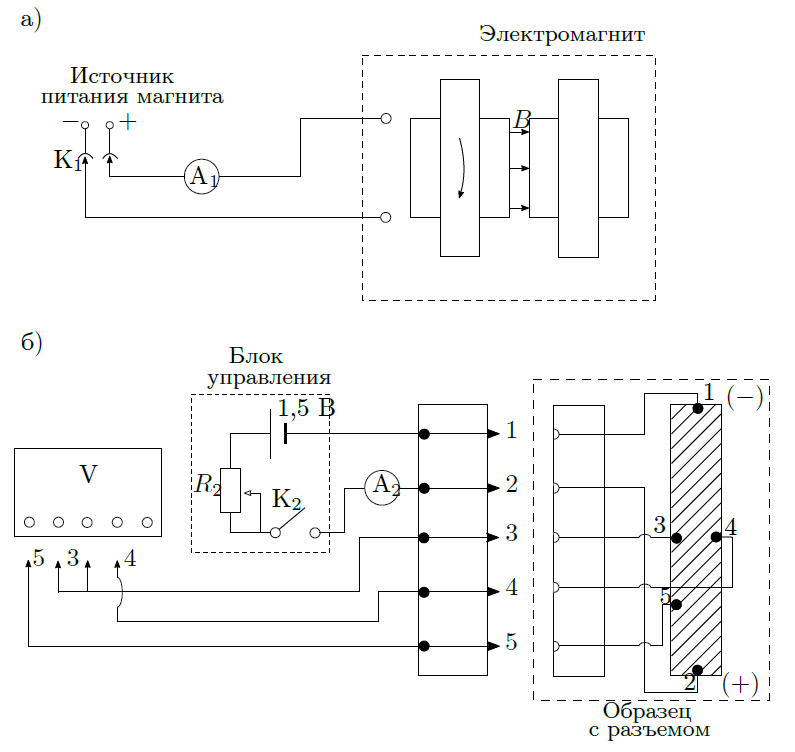
\includegraphics[width=0.55\textwidth]{Установка}
\caption{Схема экспериментальной установки для исследования эффекта Холла в полупроводниках при комнатной температуре: А$_1$, А$_2$ - амперметры для измерения тока питания электромагнита и образца соответственно; $V$ - вольтметр В7-78/1 для измерения напряжения в образце.} \label{установка}
\end{center}
\end{figure} 
\section{Результаты и их обсуждение}
\subsection*{Градуировка электромагнита}
В формуле для постоянной Холла (\ref{R_H}) присутствует индукция магнитного поля $B$, в установке есть амперметр, поэтому необходимо было связать ток с индукцией. 
Результаты измерений приведены на рисунке
\begin{figure}[h!]
\begin{center}
\includegraphics[width=\textwidth]{Градуировка}
\caption{Зависимость индукции магнитного поля $B$ от силы тока питания электромагнита $I_M$} \label{градуировка}
\end{center}
\end{figure} 
Экспериментальные значения имеют монотонный характер, график не очень похож на прямую, однако его можно приблизить квадратичной функцией: $B =  -0.412 I_M ^ 2 +1.312 I_M - 0.247$. Данное приближение и будет использоваться для определения параметров полупроводника. 
\subsection*{Измерение холловского напряжения}
При разных значениях тока через образец $I$ определено напряжение Холла в зависимости от тока через электромагнит $I_M$ (рис. \ref{U(B)}).
\begin{figure}[h!]
\begin{center}
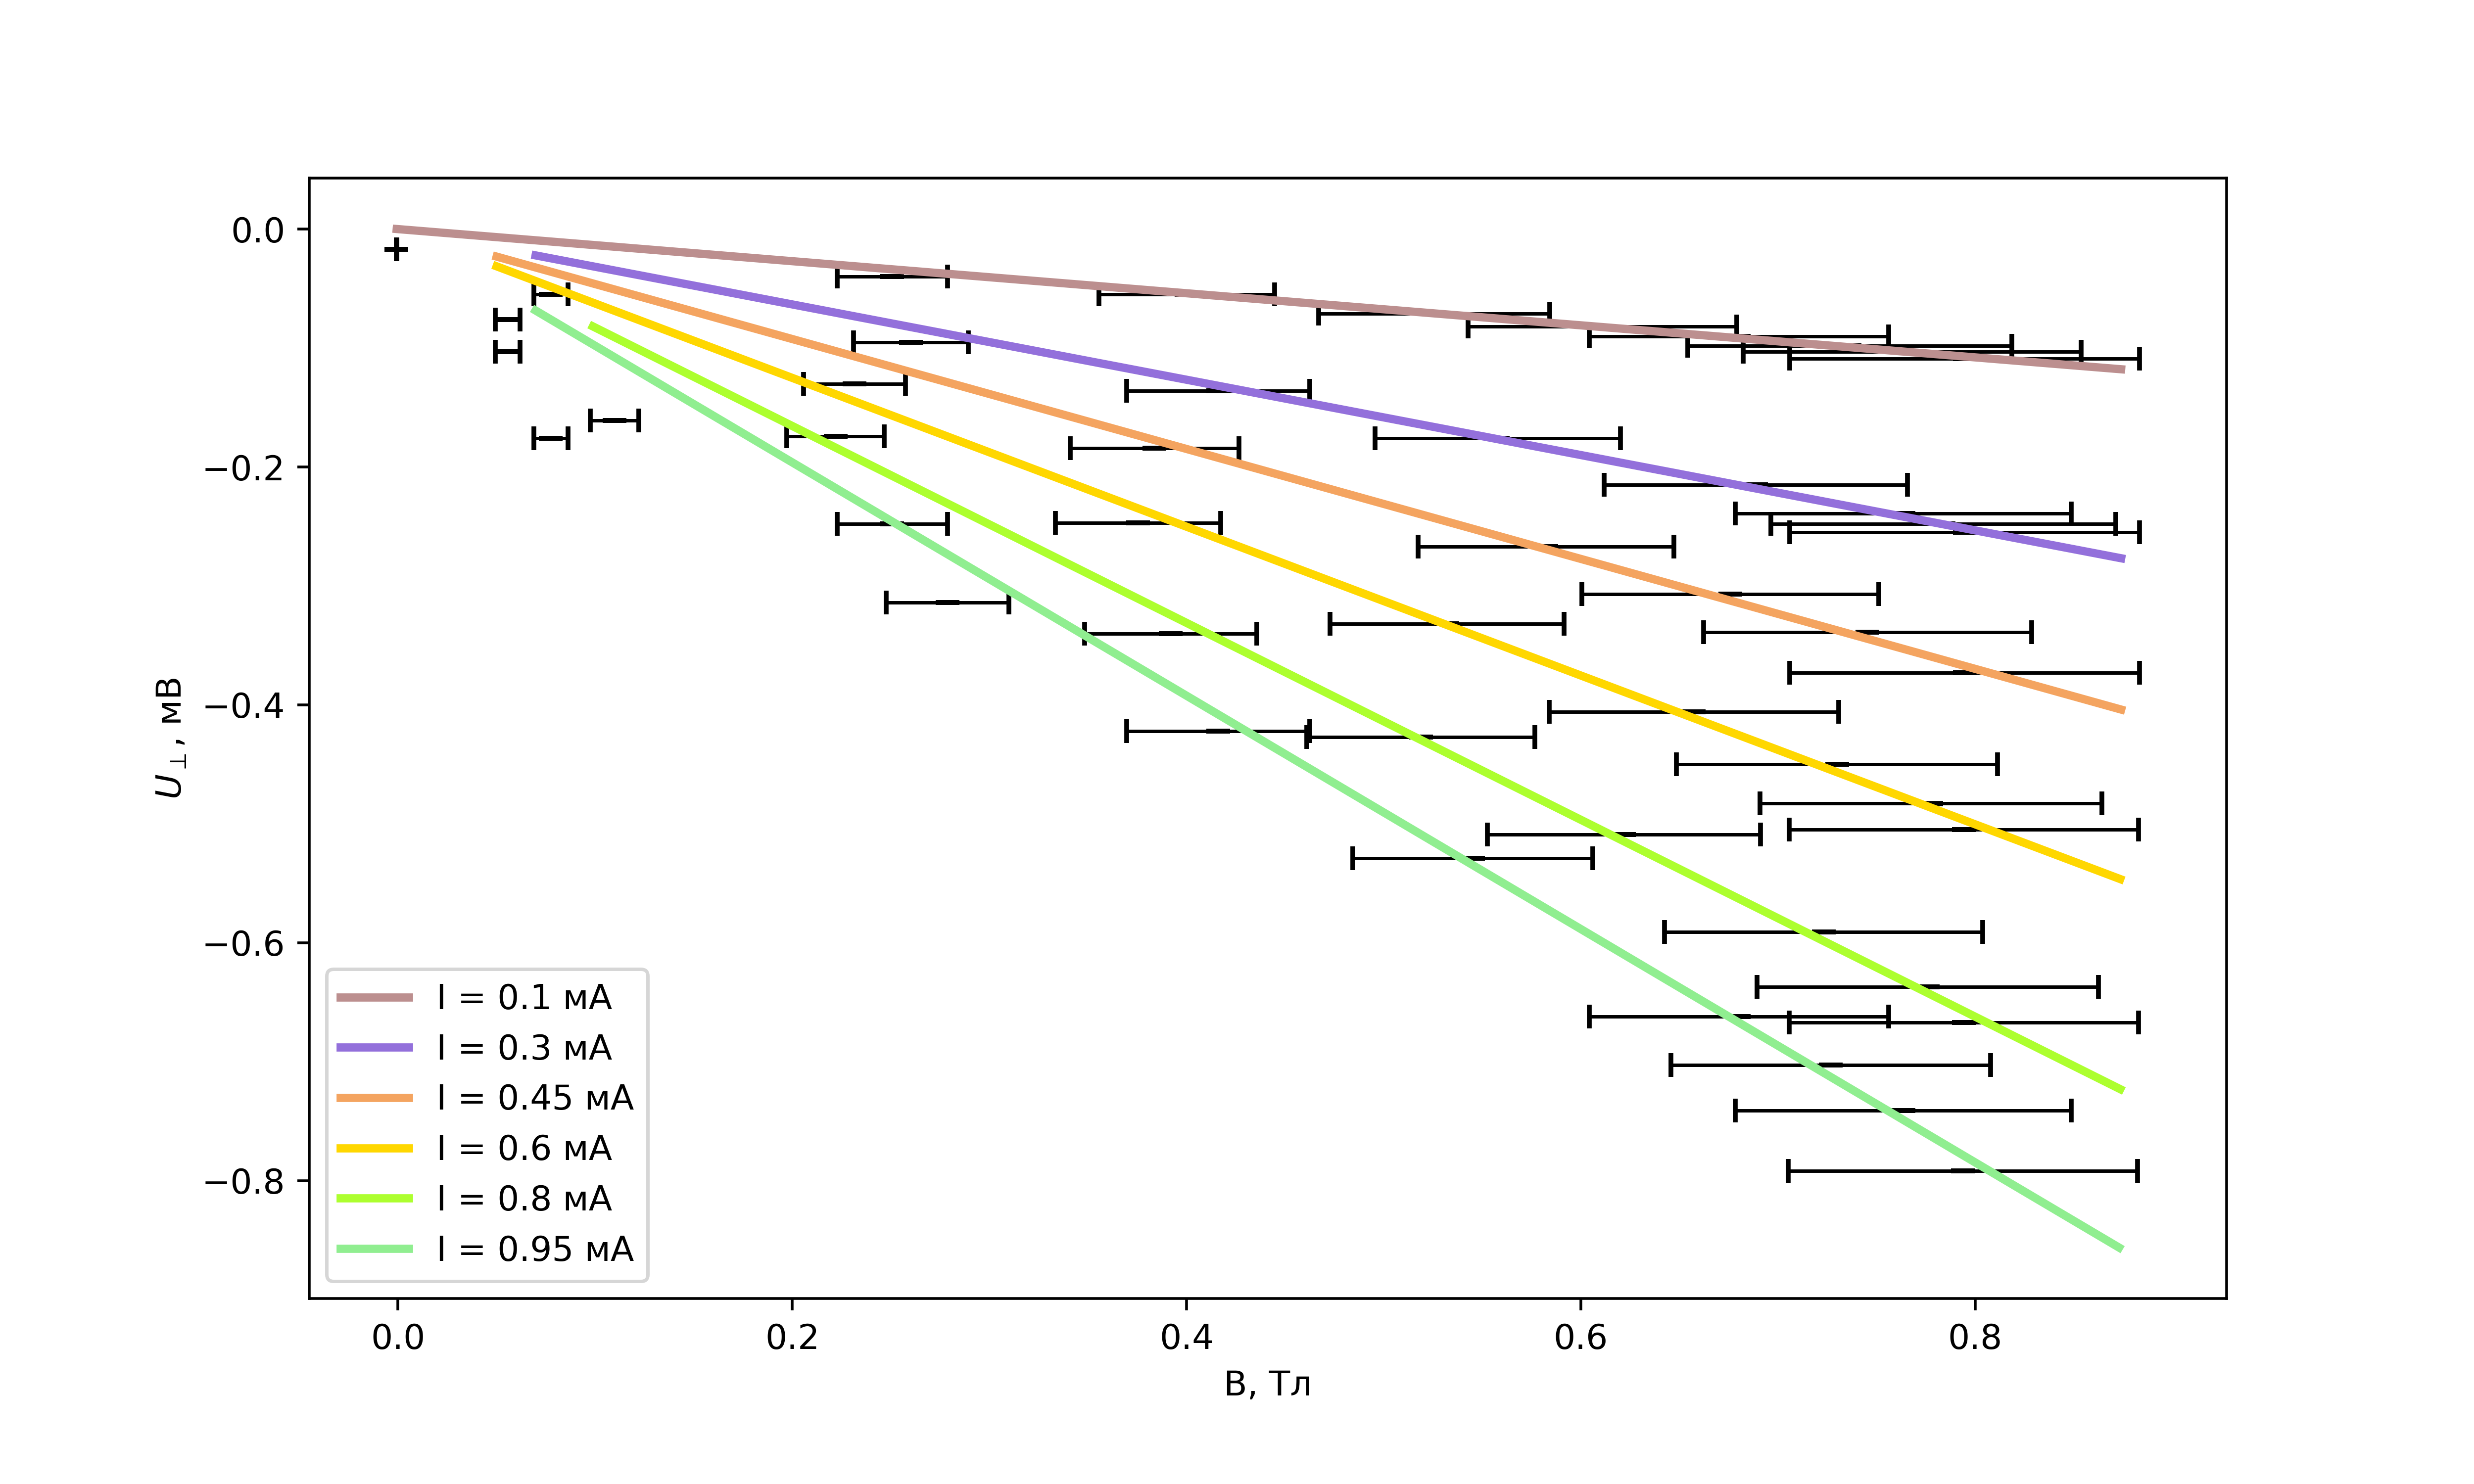
\includegraphics[width=0.95\textwidth]{E(B)}
\caption{Зависимость холловского напряжения $U_\perp$ от индукции магнитного поля в электромагните $B$} \label{U(B)}
\end{center}
\end{figure} 
Видно, что зависимость линейная, даже наблюдается прямая пропорциональность, это согласовано с теоретическими выводами (формула \ref{R_H} при фиксированном $I$). Немалые погрешности объяснимы градуировкой электромагнита на небольшом количестве точек и использовании промежуточных (между точками на графике градуировки) значений при измерении холловского напряжения.
 
Для каждого тока вычислен коэффициент наклона графика $K$ и построена его зависимость от силы тока через образец $I$ 
\begin{figure}[h!]
\begin{center}
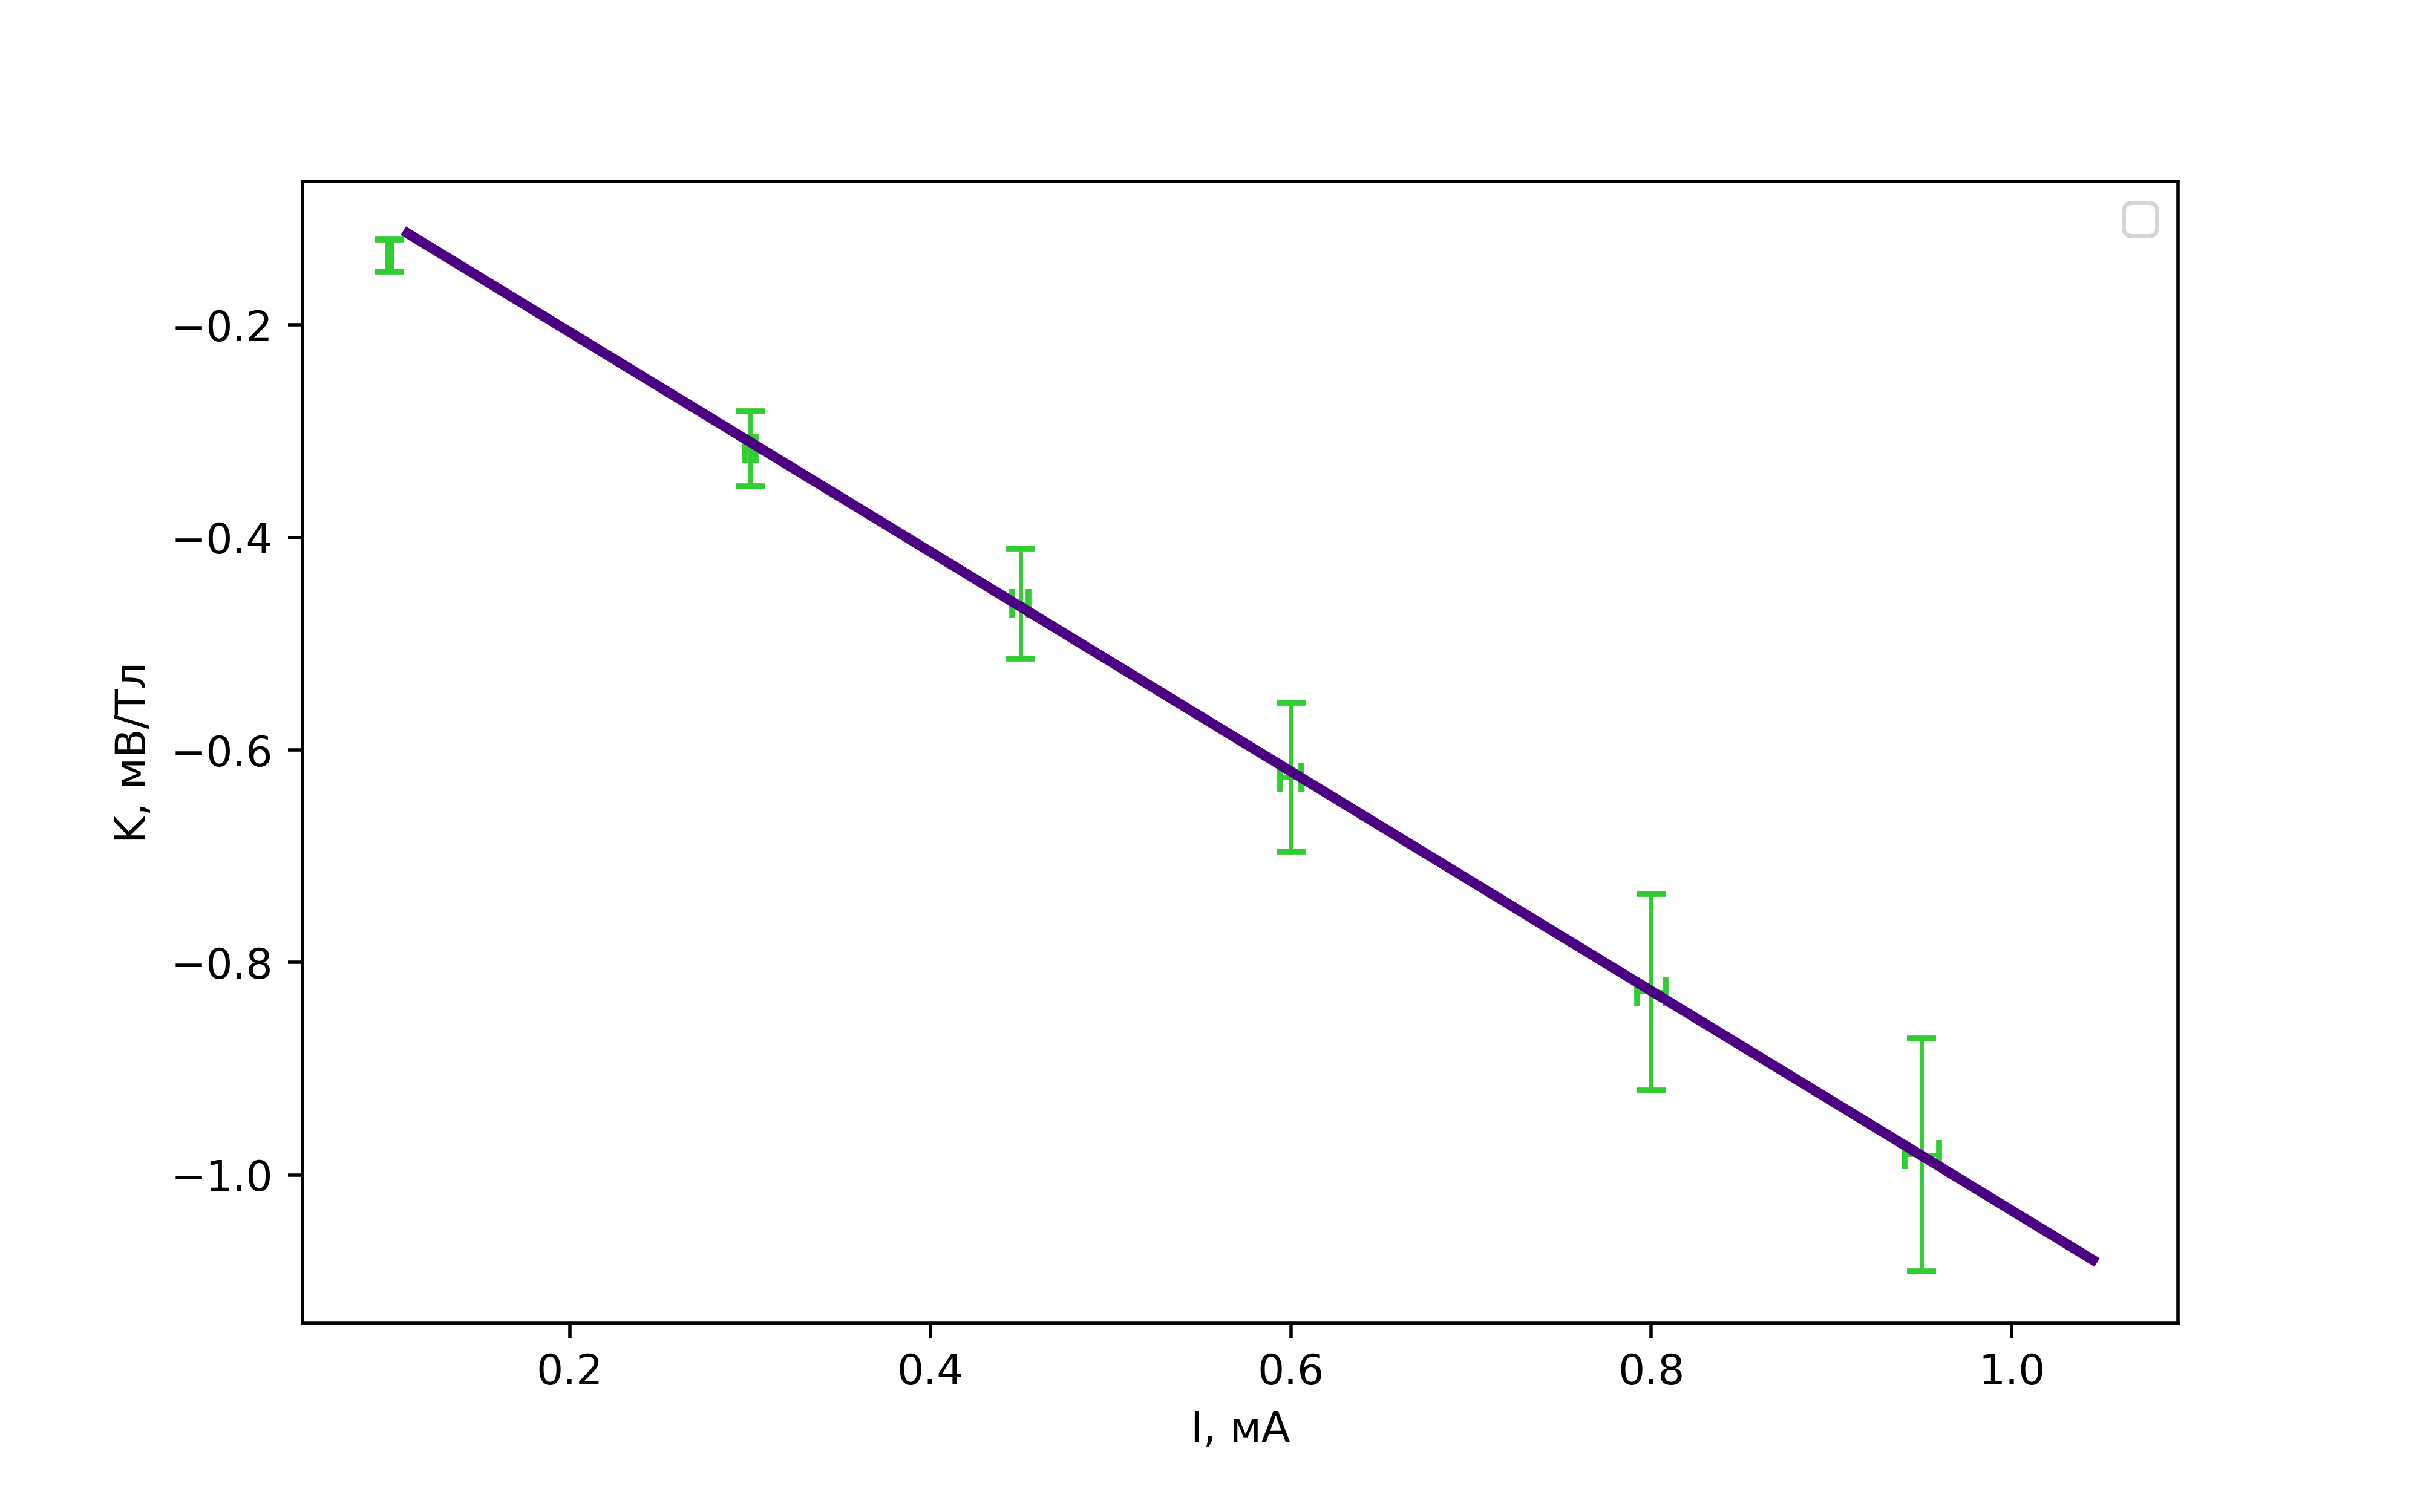
\includegraphics[width=0.95\textwidth]{K(I)}
\caption{Зависимость коэффициента наклона прямой $K=\frac{\partial U_\perp}{\partial B}$ от силы тока через образец $I$} \label{K(I)}.
\end{center}
\end{figure} 

Видно, что точки образуют прямую. Данный результат совпадает с теоретическими выкладками (формула \ref{R_H}). Из наклона данной кривой определены постоянная Холла, концентрация носителей заряда (ф-ла \ref{R_H}):
\begin{equation}
R_H = -1033 \pm 116, \hspace{0.6mm} 10^{-6} \hspace{0.6mm}\frac{м^3}{Кл}, \hspace{2mm}
n = 6.05 \pm 0.69,\hspace{0.6mm} 10^{21}\hspace{0.6mm} м^{-3}
\end{equation}

В отстуствие магнитного поля измерена проводимость материала образца:
\begin{equation}
\sigma_0 = 305 \pm 3 (Ом \cdot м)^{-1}
\end{equation}


Наконец, по формуле \ref{mu} рассчитана подвижность носителей заряда $\mu$. Однако принято использовать в общем случае подвижность частицы $b = \mu/q$ - коэффициент пропорциональности между установившейся скоростью частицы и приложенной к ней силой:
\begin{equation}
b = 3153  \pm 355 \frac{см^2}{В\cdot с} 
\end{equation}

\section{Выводы}

\hspace{4mm}1. Полученная зависимость холловского напряжения от индукции магнитного поля линейна, согласовано с теоретической зависимостью.

2. Рассчитанная зависимость коэффициента наклона графика зависимости холловского напряжения от индукции магнитного поля от силы тока через образец линейна, теоретический рассчет в данном эксперименте справедлив.

3. Вычисленное из результатов эксперимента значение подвижности частицы $b = 3153  \pm 355 \frac{см^2}{В\cdot с} $ сходится с табличным значение \cite{labnik} $b_{теор} = 3.8 \cdot 10^3 \frac{см^2}{В\cdot с}$.

4. Знак значения постоянной Холла $R_H = -1033 \pm 116, \hspace{0.6mm} 10^{-6} \hspace{0.6mm}\frac{м^3}{Кл}$ показывает, что носителями заряда в образце были электроны.




\begin{thebibliography}{}
    \bibitem{labnik}  Никулин М.Г., Попов П.В., Нозик А.А. и др. Лабораторный практикум по общей физике : учеб. пособие. В трех томах. Т. 2. Электричество и магнетизм
\end{thebibliography}
\end{document}